\usetikzlibrary{arrows.meta}
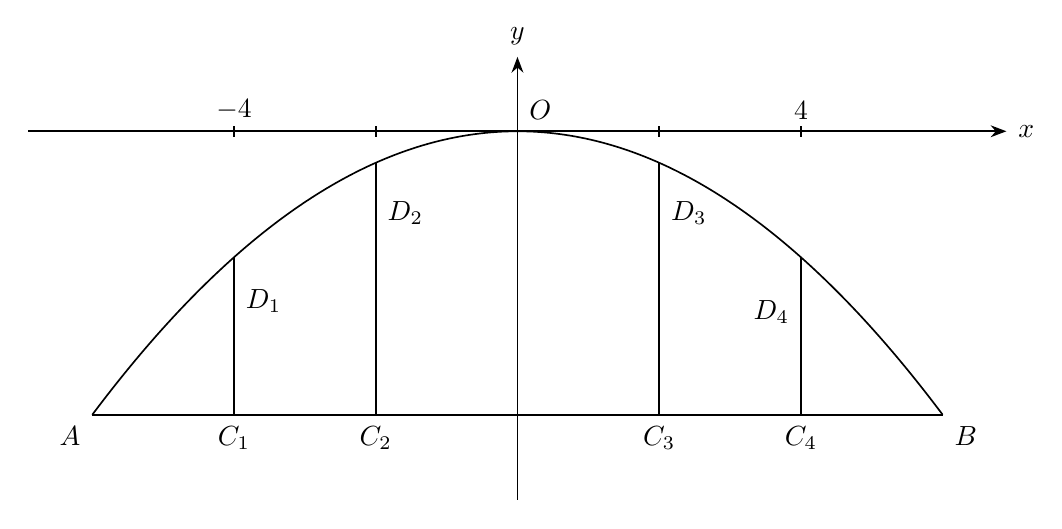
\begin{tikzpicture}[x=0.9cm,y=0.9cm,line width=.6pt,>=Stealth,font=\normalsize]
\coordinate (O) at (0,0);
\coordinate (A) at (-6,-4);
\coordinate (B) at (6,-4);
\coordinate (C1) at (-4,-4);
\coordinate (C2) at (-2,-4);
\coordinate (C3) at (2,-4);
\coordinate (C4) at (4,-4);
\coordinate (D1) at (-4,-1.7777777778);
\coordinate (D2) at (-2,-0.4444444444);
\coordinate (D3) at (2,-0.4444444444);
\coordinate (D4) at (4,-1.7777777778);
\draw[->] (-6.9,0)--(6.9,0) node[right=4pt,inner sep=0pt] {$x$};
\draw[->] (0,-5.2)--(0,1.05) node[above=4pt,inner sep=0pt] {$y$};
\draw[domain=-6:6,samples=161] plot (\x,{-\x*\x/9});
\draw (A)--(B);
\draw (C1)--(D1);
\draw (C2)--(D2);
\draw (C3)--(D3);
\draw (C4)--(D4);
\draw (-4,-0.08)--(-4,0.08);
\draw (-2,-0.08)--(-2,0.08);
\draw (2,-0.08)--(2,0.08);
\draw (4,-0.08)--(4,0.08);
\node[above right=4pt,inner sep=0pt] at (O) {$O$};
\node[below left=4pt,inner sep=0pt] at (A) {$A$};
\node[below right=4pt,inner sep=0pt] at (B) {$B$};
\node[below=4pt,inner sep=0pt] at (C1) {$C_1$};
\node[below=4pt,inner sep=0pt] at (C2) {$C_2$};
\node[below=4pt,inner sep=0pt] at (C3) {$C_3$};
\node[below=4pt,inner sep=0pt] at (C4) {$C_4$};
\node[right=4pt,inner sep=0pt] at (-4,-2.4) {$D_1$};
\node[right=4pt,inner sep=0pt] at (-2,-1.15) {$D_2$};
\node[right=4pt,inner sep=0pt] at (2,-1.15) {$D_3$};
\node[left=4pt,inner sep=0pt] at (4,-2.55) {$D_4$};
\node[above=4pt,inner sep=0pt] at (-4,0) {$-4$};
\node[above=4pt,inner sep=0pt] at (4,0) {$4$};
\end{tikzpicture}
